\chapter{Experiment and Result}
brief of experiment and result.
\section{Experiment}
Please tell how the experiment conducted from method.

\section{Result}
Please provide the result of experiment

\section{Andri Fajar Sunandhar/1164065}

\subsection{Teori}
\begin{enumerate}
\item Klasifikasi teks
	\par Klasifikasi Teks adalah salah satu tugas penting dan tipikal dalam supervised machine learning (ML). Teks dapat menjadi sumber informasi yang sangat kaya, tetapi mengekstraksi wawasan darinya bisa sulit dan memakan waktu karena sifatnya yang tidak terstruktur.
	\begin{figure}[ht]
		\centering
		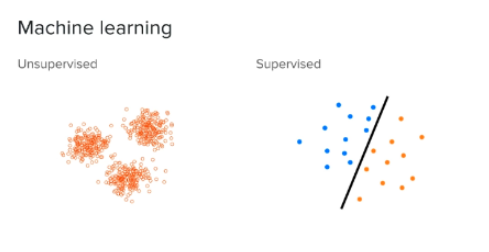
\includegraphics[scale=0.5]{figures/AFS/k1.png}
		\caption{Lusia-Klasifikasi teks}
		\label{contoh}
	\end{figure}
	
\item Mengapa Klasifikasi Bunga tidak dapat menggunakan machine learning
	\par Dikarenakan tidak semua bunga memliki ciri - ciri yang sama. Atau dalam kata lain terdapat data noise dalam klasifikasi bunga sehingga tidak bisa menggunakan machine learning.
	\begin{figure}[ht]
		\centering
		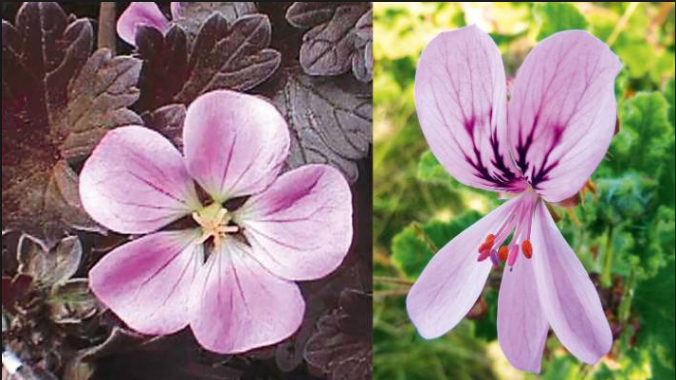
\includegraphics[scale=0.5]{figures/AFS/k2.png}
		\caption{Lusia-Klasifikasi bunga}
		\label{contoh}
	\end{figure}

\item Teknik pembelajaran mesin pada teks YouTube
	\par Kita ambil sebuah kasus yang semua orang telah ketahui dan juga pahami. Kasus tersebut yaitu perekomendasian video dari pencarian menggunakan "text / kata" di  Youtube. Pada saat menggunakan Youtube terdapat Mchine Learning yang bekerja dan memproses perintah ataupun aktivitas tersebut, dimana akan memfilter secara otomatis video yang disesuaikan dengan "keyword" yang kita masukkan sehingga memberikan keluaran video dengan keyword yang benar. Adapula pada saat kita sedang menonton video di YouTube, pada bagian sebelah kanan ( tampilan Youtube ) terdapat 'Up Next' yang menampilkan beberapa video serupa yang sedang ditonton. Dan ketika mengklik salah satu video dari baris tersebut, maka YouTube akan mengingatnya dan menggunakan kata yang tertera sebagai referensi kembali sehingga akan memberikn kemudahan pada pencarian yang lannya, Dan disitulah mesin belajar sendiri dan menyimpan data secara berkala sehingga berkembang. 

	\begin{figure}[ht]
		\centering
		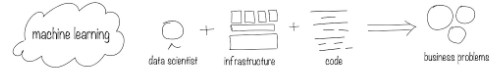
\includegraphics[scale=0.5]{figures/AFS/k3.jpeg}
		\caption{Lusia-Teknik YouTube}
		\label{contoh}
	\end{figure}

\item Vectorisasi Data
	\begin{itemize}
		\item Pembagian dan pemecahan data, dan kemudian dilakukan perhitungan datanya. Vektorisasi juga dapat dimaksudkan dengan setiap data yang mungkin dipetakan ke integer tertentu. Yang mana data tersebut dalam bentuk data vektor diperoleh dalam bentuk koordinat titik yang menampilkan, menempatkan dan menyimpan data spasial dengan menggunakan titik, garis atau area (poligon). 
	\end{itemize}
	
\item Bag of word
	\par Bag-of-words ialah sebuah gambaran sederhana digunakan dalam pengolahan bahasa alami dan pencarian informasi. Dikenal sebagai model ruang vektor. Pada model ini, tiap kalimat dalam dokumen digambarkan sebagai token, mengabaikan tata bahasa dan bahkan urutan kata namun menghitung frekuensi kejadian atau kemunculan kata dari dokumen.
	\begin{figure}[ht]
		\centering
		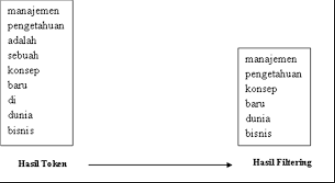
\includegraphics[scale=0.5]{figures/AFS/k4.png}
		\caption{Lusia-Bag of Word}
		\label{contoh}
	\end{figure}
	
\item TF-IDF
	\par TF-IDF atau TFIDF, adalah kependekan dari istilah frekuensi dokumen terbalik, dimana merupakan statistik numerik yang dimaksudkan untuk mencerminkan betapa pentingnya sebuah kata untuk sebuah dokumen dalam kumpulan atau kumpulan. Nilai tf-idf meningkat secara proporsional dengan berapa kali sebuah kata muncul dalam dokumen dan diimbangi dengan jumlah dokumen dalam korpus yang mengandung kata, yang membantu menyesuaikan fakta bahwa beberapa kata muncul lebih sering secara umum.
	\begin{figure}[ht]
		\centering
		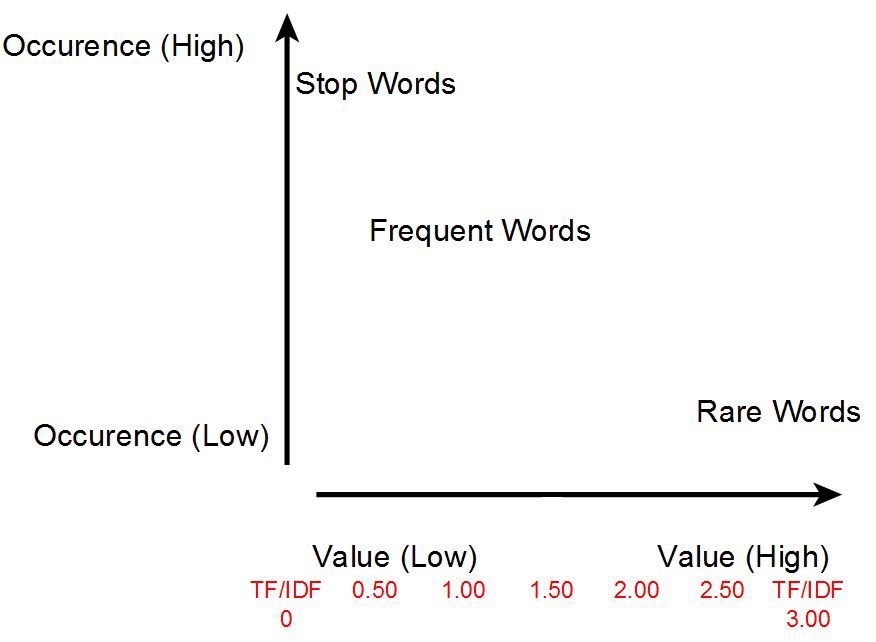
\includegraphics[scale=0.5]{figures/AFS/k5.jpeg}
		\caption{Lusia-TF IDF}
		\label{contoh}
	\end{figure}
\end{enumerate}